%%=============================================================================
%% Methodologie
%%=============================================================================

\chapter{\IfLanguageName{dutch}{Methodologie}{Methodology}}%
\label{ch:methodologie}

%% TODO: In dit hoofstuk geef je een korte toelichting over hoe je te werk bent
%% gegaan. Verdeel je onderzoek in grote fasen, en licht in elke fase toe wat
%% de doelstelling was, welke deliverables daar uit gekomen zijn, en welke
%% onderzoeksmethoden je daarbij toegepast hebt. Verantwoord waarom je
%% op deze manier te werk gegaan bent.
%% 
%% Voorbeelden van zulke fasen zijn: literatuurstudie, opstellen van een
%% requirements-analyse, opstellen long-list (bij vergelijkende studie),
%% selectie van geschikte tools (bij vergelijkende studie, "short-list"),
%% opzetten testopstelling/PoC, uitvoeren testen en verzamelen
%% van resultaten, analyse van resultaten, ...
%%
%% !!!!! LET OP !!!!!
%%
%% Het is uitdrukkelijk NIET de bedoeling dat je het grootste deel van de corpus
%% van je bachelorproef in dit hoofstuk verwerkt! Dit hoofdstuk is eerder een
%% kort overzicht van je plan van aanpak.
%%
%% Maak voor elke fase (behalve het literatuuronderzoek) een NIEUW HOOFDSTUK aan
%% en geef het een gepaste titel.

Voor het beantwoorden van de onderzoeksvraag in deze bachelorproef werd een gestructureerd plan van aanpak gevolgd. 
Het onderzoek werd opgedeeld in zes opeenvolgende fasen. 
Elke fase had een specifieke doelstelling en leverde concrete resultaten op die als basis dienden voor de volgende stappen. 
Door deze gefaseerde aanpak kon op een efficiënte 
manier toegewerkt worden naar een oplossing die aansluit bij de noden van Aquarius Zwemclub Lebbeke (AZL).

\section{Fase 1: Literatuurstudie}
De eerste fase bestond uit een literatuurstudie met als doel inzicht te krijgen in de verschillende beschikbare cloudopslagoplossingen en hun kenmerken. 
De focus lag hierbij op oplossingen die geschikt zijn voor kleinere organisaties zoals AZL, met aandacht voor integratiemogelijkheden met bestaande systemen, 
toegangsbeheer, beveiliging en kostenefficiëntie.

\textbf{Deliverable:} een overzicht van relevante cloudopslagoplossingen, gebruikt als basis voor het opstellen van een longlist in fase 3.

Deze fase was essentieel om een breed perspectief te krijgen op de markt en om oplossingen te identificeren die technisch haalbaar en betaalbaar 
zijn binnen de context van AZL.

\section{Fase 2: Requirementsanalyse}
In deze fase werd onderzocht welke functionele en niet-functionele vereisten AZL stelt aan een nieuwe cloudopslagoplossing. Dit gebeurde in nauwe samenwerking met de 
webmaster van AZL, verantwoordelijk voor het technisch beheer van de systemen.

De belangrijkste vraagstukken waren:
\begin{itemize}
    \item Efficiënt en dynamisch toegangsbeheer voor lesgevers.
    \item Bescherming van privacy door middel van duidelijke rechtenstructuren.
    \item Integratiemogelijkheden met de bestaande WordPress-website en Angular-webapplicatie.
    \item Beperkte kosten met behoud van voldoende functionaliteit.
    \item Onderhoudsvriendelijke oplossing voor de webmaster.
\end{itemize}

De vereisten werden geprioriteerd via de MoSCoW-methode, wat resulteerde in een gestructureerde lijst van eisen als richtlijn voor de verdere selectie.

\textbf{Deliverable:} een gedetailleerde en geprioriteerde lijst van vereisten.

Deze fase was noodzakelijk om te garanderen dat de gekozen oplossing perfect aansluit op de noden en werking van AZL.

\section{Fase 3: Longlist van cloudoplossingen}
Op basis van de literatuurstudie en de requirements werd een uitgebreide longlist samengesteld van potentiële cloudopslagoplossingen. Hierbij werden zowel commerciële 
als open-source alternatieven in overweging genomen.

De selectiecriteria waren:
\begin{itemize}
    \item Gebruiksvriendelijkheid voor lesgevers.
    \item Efficiënt toegangsbeheer.
    \item Sterke beveiligingsopties.
    \item Mogelijkheid tot integratie in de bestaande infrastructuur.
    \item Aangepaste kostenstructuur voor een kleine sportvereniging.
\end{itemize}

\textbf{Deliverable:} een longlist van mogelijke oplossingen die voldoen aan de vooropgestelde criteria.

Deze brede verkenning garandeerde dat geen potentieel relevante oplossingen over het hoofd werden gezien.

\section{Fase 4: Shortlist en selectie}
Uit de longlist werd vervolgens een shortlist opgesteld. Via een vergelijkende analyse werden de voor- en nadelen van de geselecteerde oplossingen systematisch in 
kaart gebracht.

De belangrijkste criteria bij de vergelijking waren:
\begin{itemize}
    \item Toegangsbeheer en gebruiksgemak.
    \item Integratiegraad met de bestaande systemen.
    \item Beveiliging en privacy.
    \item Totaalkost en onderhoudsbehoefte.
\end{itemize}

Op basis van deze analyse werd de meest geschikte oplossing geselecteerd. 
Back-upopties werden voorzien voor het geval de primaire keuze niet voldeed tijdens de testfase.

\textbf{Deliverable:} een tabel met de vergelijking van de alternatieven en de definitieve selectie van de beste oplossing.

Deze fase maakte het mogelijk om onderbouwd en objectief tot een keuze te komen die aan alle prioritaire vereisten voldeed.

\section{Fase 5: Proof of Concept (PoC)}
In deze fase werd de geselecteerde oplossing geïmplementeerd als een proof of concept. 
Het doel was om de werking van de oplossing in de praktijk te toetsen en te evalueren.

De PoC bestond uit:
\begin{itemize}
    \item Integratie van de cloudopslag met de bestaande infrastructuur.
    \item Instellen van toegangsbeheer volgens de vooraf bepaalde vereisten.
    \item Testperiode waarbij lesgevers en de webmaster de oplossing gebruikten.
\end{itemize}

Gedurende twee weken werd feedback verzameld over gebruiksgemak, beheerbaarheid en betrouwbaarheid. 
Deze feedback werd geanalyseerd en gebruikt om verbeterpunten te identificeren.

\textbf{Deliverable:} een werkend prototype van de gekozen oplossing, inclusief gebruikersfeedback en optimalisatievoorstellen.

Deze fase was cruciaal om te verifiëren of de gekozen oplossing daadwerkelijk toepasbaar is binnen AZL.

\section{Fase 6: Evaluatie en conclusies}
Na afronding van de PoC werd een uitgebreide evaluatie uitgevoerd. Hierbij werd nagegaan in hoeverre de oplossing 
voldeed aan de vooraf opgestelde vereisten en hoe deze zich verhield tot de oorspronkelijke problemen met Dropbox.

Belangrijke aandachtspunten waren:
\begin{itemize}
    \item Vermindering van de administratieve last.
    \item Verbetering van de toegankelijkheid voor lesgevers.
    \item Betrouwbaarheid en veiligheid van de oplossing.
\end{itemize}

Op basis van de evaluatie werden aanbevelingen geformuleerd voor een eventuele definitieve implementatie bij AZL.

\textbf{Deliverable:} een eindrapport met conclusies en aanbevelingen.

\section{Visualisatie en tijdsplanning}
De methodologie werd gepland over een periode van tien weken, van 07/03/2025 tot 23/05/2025. 
De fasen volgden elkaar logisch op, waarbij elke fase afhankelijk was van de resultaten van de vorige stap. 
De tijdsplanning werd weergegeven in een Gantt Chart en zorgde voor een duidelijke opvolging van de voortgang.

In de eerste weken lag de nadruk op onderzoek en analyse. De laatste weken stonden in het teken van implementatie, testen en evaluatie. 
Deze gefaseerde aanpak garandeerde een grondige en betrouwbare uitwerking van de bachelorproef.

\begin{figure}[h!]
    \centering
    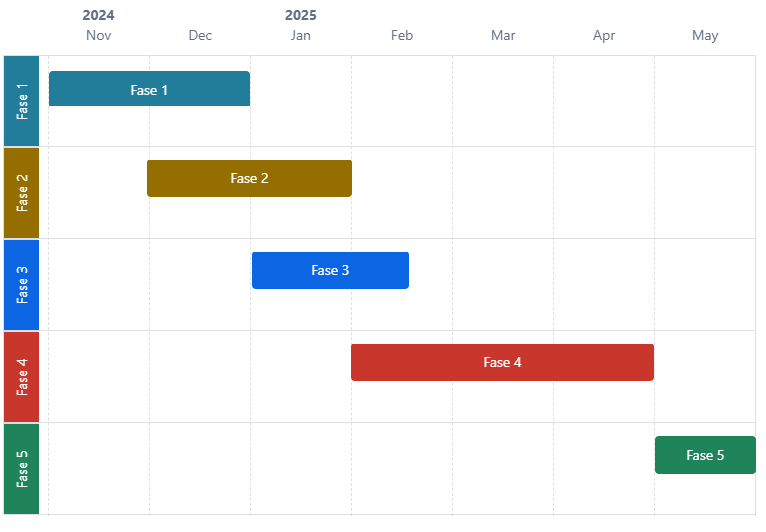
\includegraphics[width=.5\textwidth]{../graphics/Chart-Tijd-Visualisatie.png}
    \caption{Tijdsplanning van het project}
    \label{fig:tijdsplanning}
\end{figure}